% Chapter 4

\chapter{Proposed Methodology} % Main chapter title

\label{Chapter4} % For referencing the chapter elsewhere, use \ref{Chapter4} 

\lhead{Chapter 4. \emph{ Proposed Methodology }} % This is for the header on each page - perhaps a shortened title

%-----------------------------------------------------------------------
In the previous chapter, we have discussed about the various machine learning techniques that are generally used  for Segmentation and Classification of Brain Tumor from MRI Images. We  have  used  some  of  these  techniques  on  our  dataset and  then  we  have  applied  our  model  on  the  dataset  to  compare  their  accuracy.   Before  these techniques are applied we have followed a few steps to process the data to remove null values and handle missing data from the dataset, this process is termed as data preprocessing.

This describes the materials, the source from which the brain image data collected and the algorithms for brain MRI segmentation and feature extraction. The methodology proposed includes application on brain MRI images of 256 × 256, 512 × 512 pixel size on dataset. It is converted into gray scale for further enhancement. The following discussion deals with implementation of algorithm.

Proposed method having following important blocks they are
\begin{enumerate}
    \item Pre-processing
    \item Patch Extraction
    \item Patch Pre-processing
    \item Feature Extraction
    \item CNN Training & Testing
    \item Performance
\end{enumerate}

The main Objective of this project is to accurately segment the brain abnormal portion by using the conventional neural network. A Convolutional Neural Network is used to segment the brain abnormal image by performing testing and training separately. To measure Sensitivity analysis includes true positive (TP), true negative (TN), false positive (FP), false negative (FN) etc. Pre-processing includes the removal of noise or unwanted distortion from the input image. It can help to increase the quality of the performance. Next step is to convert the image into patches or blocks to perform further operations. As we know we are using the neural network, we have to perform training as well as testing phases separately. For performing NNT training features should be extracted to learn neural network. Sensitivity analysis is used for performance anal


% \begin{figure}[h!]
%     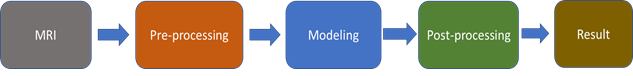
\includegraphics[scale=0.8]{Figures/p_model.png}
%     \caption{Proposed Methodoloy steps}
%     \label{fig:p_methodology}
% \end{figure}

\section{Pre-processing}
Preprocessing is one of the important steps in the image processing. In this work, mainly the preprocessing is done to perform the skull removal operation. By the combination of thresholding an morphological operation like dilation and erosion it is performed. A potential confounder in various image analysis tasks in the presence of a low-frequency intensity non-uniformity present in the image data also known as bias, in homogeneity, illumination non-uniformity, or gain field. 
N4ITK method is applied to MRI images to correct bias field distortion. MRI images are altered by the bias field distortion. However, this is not enough to ensure that the intensity distribution of a tissue type is in a similar intensity scale across different subjects for the same MRI sequence, which is an explicit or implicit assumption in most segmentation methods In fact, it can vary even if the image of the same patient is acquired in the same scanner in different time points, or in the presence of a pathology So, to make the contrast and intensity ranges more similar across patients and acquisitions, apply the intensity normalization a two-step method wherein all images (independent of patients and the specific brand of the MR scanner used) can be transformed in such a way that for the same protocol and body region, in the transformed images similar intensities will have similar tissue meaning.
In this intensity normalization method, a set of intensity landmarks are learned for each sequence from the training set and are chosen for each MRI sequence as described in represents the intensity at the percentile.

After training, the intensity normalization is accomplished by linearly transforming the original intensities between two landmarks into the corresponding learned landmarks. In this way, the histogram of each sequence is more similar across subjects. After normalizing the MRI images, we compute the mean intensity value and standard deviation across all training patches extracted for each sequence. Then, we normalize the patches on each sequence to have zero mean and unit variance.


    \subsection{Train/Test Split}
    The data we use is usually split into training data and test data. The training set contains a known output and the model learns on this data in order to be generalized to other data later on. We have the test dataset (or subset) in order to test our model’s prediction on this subset. The proportions generally used is 70\% in training and 30\% in testing data.  The training set and test set is divided into two parts x and y.

      \begin{figure}[h!]
        \centering
         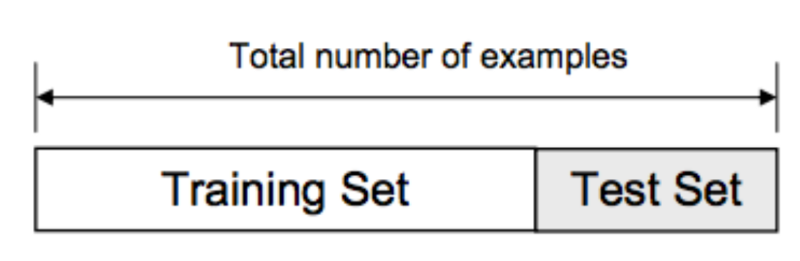
\includegraphics[scale=0.3]{Figures/split.png}
        \caption{Train/Test Split}
      \end{figure}
      
      \begin{itemize}
          \item Overfitting: 
          Overfitting means that model we trained has trained “too well” and is now, well, fit too closely to the training dataset. This usually happens when the model is too complex (i.e. too many features/variables compared to the number of observations). This model will be very accurate on the training data but will probably be very not accurate on untrained or new data. It is because this model is not generalized (or not AS generalized), meaning you can generalize the results and can’t make any inferences on other data, which is, ultimately, what you are trying to do. Basically, when this happens, the model learns or describes the “noise” in the training data instead of the actual relationships between variables in the data. This noise, obviously, isn’t part in of any new dataset, and cannot be applied to it.
          
          \item Underfitting: 
          In contrast to overfitting, when a model is underfitted, it means that the model does not fit the training data and therefore misses the trends in the data. It also means the model cannot be generalized to new data. As you probably guessed (or figured out!), this is usually the result of a very simple model (not enough predictors/independent variables). It could also happen when, for example, we fit a linear model (like linear regression) to data that is not linear. It almost goes without saying that this model will have poor predictive ability (on training data and can’t be generalized to other data)
      \end{itemize}
      
      \begin{figure}[h!]
        \centering
         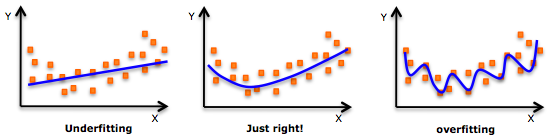
\includegraphics[scale=0.5]{Figures/over_under.png}
        \caption{An example of overfitting, underfitting and a balanced model}
      \end{figure}
      
      \subsection{Patch Extraction & Patch Pre-Processing}
      
    In patch extraction step, the images are converted into small blocks of size3x3. By converting into the patch, we can get more local information which can help to determine the tumor portion of the image. In this work, sliding windowing technique is used to extract the pixel blocks. By using sliding window more accurate information about the region we can estimate. In patch preprocessing the blocks will be converted into an array to find out the features of the local region.      
  
  
  
%   \begin{figure}
%       \centering
%       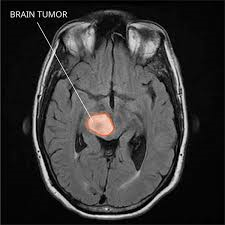
\includegraphics{Chapters/glioma.png}
%       \caption{Glioma}
%       \label{fig:my_label}
%   \end{figure}
%   \begin{figure}
%       \centering
%       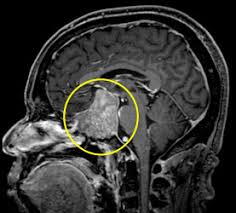
\includegraphics{Chapters/pituitary.png}
%      \caption{Pituitary}
%       \label{fig:my_label}
%   \end{figure}
    %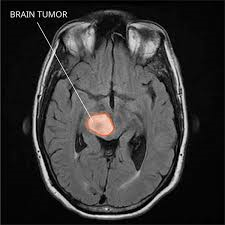
\includegraphics{Chapters/glioma.png}
   % \caption{Glioma}
    %\label{fig:my_label}
    
    %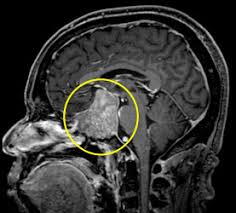
\includegraphics{Chapters/pituitary.png}
   %\caption{Pituitary}
    %\label{fig:my_label}
  %\end{figure}
%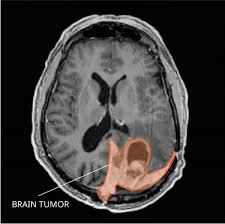
\includegraphics{Chapters/meningioma.png}
%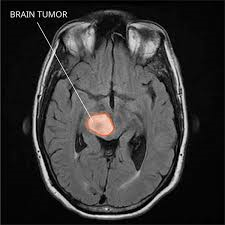
\includegraphics{Chapters/glioma.png}\\


\subsection{Image Segmentation}

The segmentation is a process where the image is partitioned into different regions. Let an entire region of image be represented by S. Segmentation process can be viewed as partition of S into p subregions like S1, S2, S3, …Sp. Certain conditions has to satisfied such as the segmentation must be intact; that is each and every pixel should be within the region, every points in the regions should be connected in some sense, regions should be disjoint, etc.

\subsection{Region growing}

Region growing is grouping of pixels or subregions into larger regions based on certain criteria. The main aim was to select a ‘seed’ points and attach each of these seed to those neighboring pixels having identical properties to grow region. A set of seeds was taken as input within the image and marked the objects to be segmented. The region grows iteratively by estimating all unallocated neighboring pixels of the region. The similarity was the measure of difference between pixel’s intensity value and the region’s mean, δ. The pixel with the smallest difference measured this way was allocated to the respective region. This was continued until all pixels were allocated to a region. Seeded region growing requires seeds as additional input. The results depend on the selection of seeds. The measurement was based on mean value of the pixel intensity. The image gets segmented; this image was used to identify the desired tumor region.

\section{Morphological Operation}

    Watershed transformation additionally called, as watershed method is an effective mathematical morphological tool for the image segmentation. It is more prevalent in the fields like biomedical and medical image processing, and computer vision. In topography, watershed means the edge that partitions area drained by diverse river system. If image is viewed as geological landscape, the watershed lines find out boundaries which separate image regions. The watershed transform figures catchment basins and ridge lines (otherwise called watershed lines), where catchment basins relating to image regions and ridge lines identifying with region boundaries. Segmentation by watershed embodies many of the concepts of the three techniques such as threshold based, edge based and region based segmentation.
    
    Watershed algorithms based on watershed transformation have mainly two classes. The first class contains the flooding based watershed algorithms and it is a traditional approach where as the second class contains rain falling based watershed algorithms. Many algorithms have been proposed in both classes but connected components based watershed algorithm shows very  good performance compared to all others. It comes under the rain falling based watershed algorithm approach. It gives very good segmentation results, and meets the criteria of less computational complexity.
    \newpage
    The steps for the operations are as follows:
  
    \begin{figure}[h!]
        \centering
            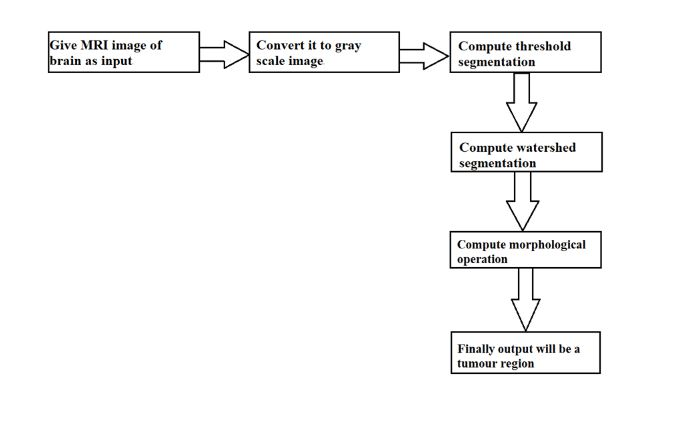
\includegraphics[scale=0.5]{Figures/water.png}
            \caption{Steps for Watershed & Morphological operation}
            \label{fig:my_label}
     \end{figure}
    
   
   \begin{enumerate}
       \item Give MRI image of brain as input
            Load the first MRI from the dataset. fig.4.6, shows the original image from which the tumor has to be detected  
        
            \begin{figure}[h!]
                 \centering
                 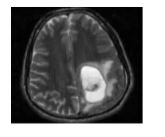
\includegraphics[scale=0.5]{Figures/11.png}
                 \caption{MRI Image}
                 \label{fig:my_label}
           \end{figure}
        \item Convert it to gray scale image
            The original image contains some RGB value. It has to be converted
            \begin{figure}[h!]
                \centering
                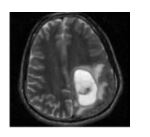
\includegraphics[scale=0.5]{Chapters/12.png}
                \caption{RGB to Gray converted image}
                \label{fig:RGB to Gray converted image}
            \end{figure}
        \item Compute threshold segmentation
            Threshold segmentation is one of the simplest segmentation systems. The input gray scale image is changed into a binary image.
            \begin{figure}[h!]
                \centering
                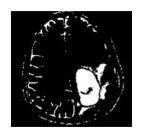
\includegraphics[scale=0.5]{Figures/13.png}
                \caption{Binary image}
                \label{fig:Binary image}
            \end{figure}
        \item Compute watershed segmentation
            Pixels falling under comparative intensities are assembled together. It is a decent segmentation system for separating a image to partition a tumor from the image. 
            After changing over the image in the binary format, some morphological operations are applied on it. The motivation behind the morphological operator is to discrete the tumor part of the image.
        \item Finally output will be a tumour region
        The fig. 5.7 shows the final extracted brain tumor
            \begin{figure}[h!]
                \centering
                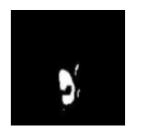
\includegraphics[scale=0.5]{Figures/14.png}
                \caption[Segmented Tumor Mask]{Segmented Tumor Mask}
                \label{fig:Segmented Tumor Mask}
            \end{figure}
   
   \end{enumerate}
 
\section{Feature Extraction}
It is the process of collecting higher-level information of an image such as shape, texture, color, and contrast.  It is used effectively to improve the accuracy of diagnosis system by selecting prominent features.

The statistics feature formula for features we have used are as follows:

\begin{enumerate}
    \item Mean (M): The mean of an image is calculated by adding all the pixel values of an image divided by the total number of pixels in an image.
    \item Standard Deviation (SD):  The standard deviation is the second central moment describing probability distribution of an observed population and can serve as a measure of in homogeneity. A higher value indicates better intensity level and high contrast of edges of an image.
    \item Entropy (E): Entropy is calculated to characterize the randomness of the textural image and is defined as corresponding states of intensity level which individual pixels can adapt. It is used in the quantitative analysis and evaluation image details, the entropy value is used as it provides better comparison of the image details.
    \item Energy (En): Energy can be defined as the quantifiable amount of the extent of pixel pair repetitions.
    \item Skewness ($S_k$): Skewness is a measure of symmetry or the lack of symmetry. The skewness of a random variable $X$ is denoted as $S_k(X)$.
    \item Kurtosis ($K_u_r_t$): The shape of a random variable’s probability distribution is described by the parameter called Kurtosis. For the random variable $X$, the Kurtosis is denoted as $K_u_r_t(X)$
    \item RMS(Root Mean Square): It is another way of calculating mean for set of pixels
    \item Variance: It is a measurement of the spread between pixels in an Image. The square root of variance is the standard deviation (σ).
\end{enumerate}

\section{Classification}
   
   Here we used many type of machine learning algorithm to
   classify the MRI of brain tumor and compare their performing, they are SVM, Decision tree, Naive Bayes, MLP, Logistic Regression.
  
\subsection{SVM}

  “Support Vector Machine” (SVM) is a supervised machine learning algorithm which can be used for both classification or regression challenges. However,  it is mostly used in classification problems. In this algorithm, we plot each data item as a point in n-dimensional space (where n is number of features you have) with the value of each feature being the value of a particular coordinate. Then, we perform classification by finding the hyper-plane that differentiate the two classes very well.
  
  
  \begin{figure}[h!]
  \centering
    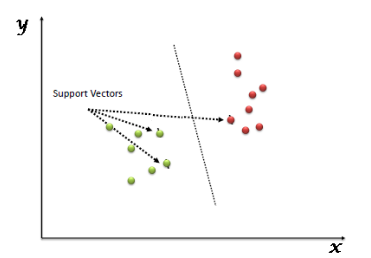
\includegraphics[scale=0.5]{Figures/svm11.png}
    \caption[SVM]{SVM}
    \label{fig:my_label}
  \end{figure}
  
  Support Vectors are simply the co-ordinates of individual observation. Support Vector Machine is a frontier which best segregates the two classes (hyper-plane/line).
  
  \subsubsection{How it Works}
  
  Above, we got accustomed to the process of segregating the two classes with a hyper-plane. Now the burning question is “How can we identify the right hyper-plane?”.
  
    \begin{enumerate}
        \item Identify the right hyper-plane(Scenario-1)
        Here, we  have three hyper-planes (A,B and C). Now, identify the right hyper-plane to classify star and circle.
            
        You need to remember a thumb rule to identify the right hyper-plane: “Select the hyper-plane which segregates the two classes better”. In this scenario, hyper-plane “B” has excellently performed this job.
        \item Identify the right hyper-plane(Scenario-2): 
        Here, we have three hyper-planes (A, B and C) and all are segregating the classes well. Now, How can we identify the right hyper-plane?
            \begin{figure}[h!]
                \centering
                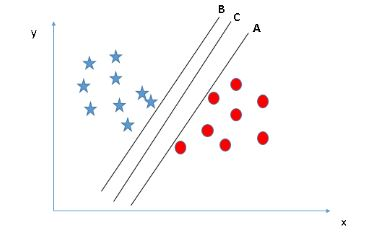
\includegraphics[scale=0.5]{Figures/svm13.png}
                \caption[Identify the right hyper-plane 2]{Identify the right hyper-plane 2}
                \label{fig:my_label}
            \end{figure}
        \item Here, maximizing the distances between nearest data point (either class) and hyper-plane will help us to decide the right hyper-plane. This distance is called as Margin. Let’s look at the below snapshot:
            \begin{figure}[h!]
                \centering
                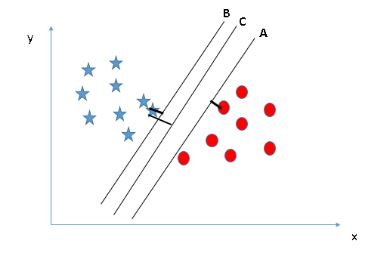
\includegraphics[scale=0.5]{Figures/svm14.png}
                \caption[Identify the right hyper-plane 2.1]{Identify the right hyper-plane 2.1}
                \label{fig:my_label}
            \end{figure}
        Above, we can see that the margin for hyper-plane C is high as compared to both A and B. Hence, the name of the right hyper-plane as C. Another lightning reason for selecting the hyper-plane with higher margin is robustness. If we select a hyper-plane having low margin then there is high chance of miss-classification.
        \item Identify the right hyper-plane (Scenario-3): Here use the rules as discussed in previous section to identify the right hyper-plane.
            \begin{figure}[h!]
                \centering
                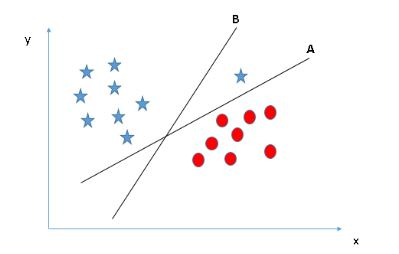
\includegraphics[scale=0.5]{Figures/svm15.png}
                \caption[Identify the right hyper-plane 3]{Identify the right hyper-plane 3}
                \label{fig:my_label}
            \end{figure}
        Some of us may have selected the hyper-plane B as it has higher margin compared to A. But, here is the catch, SVM selects the hyper-plane which classifies the classes accurately prior to maximizing margin. Here, hyper-plane B has a classification error and A has classified all correctly. Therefore, the right hyper-plane is A.
        
    \end{enumerate}

   
   \underline{The advantages of using SVM are listed as follows}:
   
   \begin{enumerate}
       \item SVM include high accuracy, elegant mathematical tractability, and direct geometric interpretation.
       \item It has few tunable parameters.
       \item Training often involves convex optimization. Hence, solutions are global and usually unique, thus avoiding the convergence to local minima exhibited by other statistical learning systems, such as neural networks.
   \end{enumerate}
   
\subsection{Decision Tree}

  Decision Trees are a type of Supervised Machine Learning (that is explain what the input is and the corresponding output is in the training data) where the data is continuously split according to a certain parameter. The tree can be explained by two entities, namely decision nodes and leaves. The leaves are the decisions or the final outcomes. And the decision nodes are where the data is split.
  
    \begin{figure}[h!]  
        \centering
        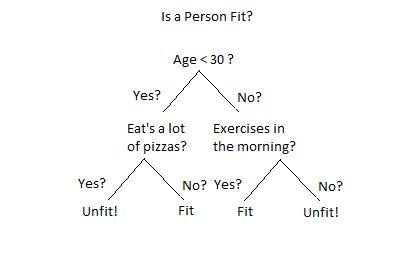
\includegraphics[scale=0.7]{Figures/decisiontree1.JPG}
        \caption{Decision Tree}[Decision Tree]
        \label{fig:my_label}
    \end{figure}
   
   An example of a decision tree can be explained using above binary tree. If you want to predict whether a person is fit given their information like age, eating habit, and physical activity, etc. The decision nodes here are questions like ‘What’s the age?’, ‘Does he exercise?’, ‘Does he eat a lot of pizzas’? And the leaves, which are outcomes like either ‘fit’, or ‘unfit’. In this case this was a binary classification problem (yes no type problem).
   
   There are two main types of Decision Trees:
   
   \begin{enumerate}
       \item Classification trees (Yes/No types):
       What we have seen above is an example of classification tree, where the outcome was a variable like ‘fit’ or ‘unfit’. Here the decision variable is Categorical.
       \item Regression trees (Continuous data types):
       Here the decision or the outcome variable is Continuous, e.g. a number like 123.
   \end{enumerate}
   
   \underline{Advantages}:
   
   \begin{enumerate}
       \item Minimum requirement of data cleaning
       \item Method is Non Parametric
       \item Can be used in Data exploration
       \item Constraint of Data type not present
       \item Can be easily Understandable
   \end{enumerate}
   
  \underline{Disadvantages}:
  
  \begin{enumerate}
      \item Over fitting
      \item Not fit for continuous variables
  \end{enumerate}
    
   \textbf{\underline{Working}}:
    
    The best algorithm to construct decision tree  is ID3 Algorithm. ID3 Stands for Iterative Dichotomiser 3.
    
    \textbf{Entropy}
    
    Entropy, also called as Shannon Entropy is denoted by H(S) for a finite set S, is the measure of the amount of uncertainty or randomness in data.
    
    
    \begin{figure}[h!]
        \centering
        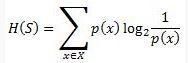
\includegraphics[scale=0.8]{Figures/a1.png}
    \end{figure}
   
   Intuitively, it tells us about the predictability of a certain event. Example, consider a coin toss whose probability of heads is 0.5 and probability of tails is 0.5. Here the entropy is the highest possible, since there’s no way of determining what the outcome might be. Alternatively, consider a coin which has heads on both the sides, the entropy of such an event can be predicted perfectly since we know beforehand that it’ll always be heads. In other words, this event has no randomness hence it’s entropy is zero.
   
   \textbf{Information Gain}

   Information gain is also called as Kullback-Leibler divergence denoted by IG(S,A) for a set S is the effective change in entropy after deciding on a particular attribute A. It measures the relative change in entropy with respect to the independent variables.
  
   
   \begin{figure}[h!]
        \centering
        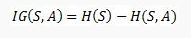
\includegraphics[scale=0.8]{Figures/a2.png}
   \end{figure}
  
   Alternatively,
   
   \begin{figure}[h!]
       \centering
         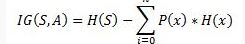
\includegraphics[scale=0.8]{Figures/a3.png}
   \end{figure}
  
   where IG(S, A) is the information gain by applying feature A. H(S) is the Entropy of the entire set, while the second term calculates the Entropy after applying the feature A, where P(x) is the probability of event x.
  
\subsection{Naive Bayes}
  
  Naive Bayes is a machine learning algorithm for classification problems. It is based on Bayes’ probability theorem. It is primarily used for text classification which involves high dimensional training data sets. A few examples are spam filtration, sentimental analysis, and classifying news articles.
  The Naive Bayes algorithm is called "naive" because it makes the assumption that the occurrence of a certain feature is independant of the occurance of other feature. 
  
  A Naive Bayes Classifier is a supervised machine-learning algorithm that uses the Bayes’ Theorem, which assumes that features are statistically independent. The theorem relies on the naive assumption that input variables are independent of each other, i.e. there is no way to know anything about other variables when given an additional variable. Regardless of this assumption, it has proven itself to be a classifier with good results.
  
  Naive Bayes Classifiers rely on the Bayes’ Theorem, which is based on conditional probability or in simple terms, the likelihood that an event (A) will happen given that another event (B) has already happened. Essentially, the theorem allows a hypothesis to be updated each time new evidence is introduced. The equation below expresses Bayes’ Theorem in the language of probability:
  
    \begin{figure}[h!]
        \centering
        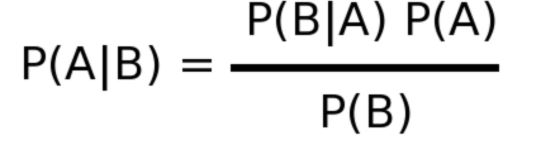
\includegraphics[scale=0.5]{Figures/eq2.png}
    \end{figure}

\subsection{MLP}
   
    The multi-layer perceptron is a feed forward neural network consisting of an input layer of nodes, followed by two or more layers of perceptron, the last of which is the output layer. The layers between the input layer and output layer are referred to as hidden layers. It has a lot of successful applications in solving complex problems in the real world, consisting of non-linear decision boundaries.
    
    MLP does not have any cycles and the output depends only
   on the input samples therefore it is named feed forward. It depends on supervised learning. Learning process conducted by changing the connection weights after handling each piece of data, based on the amount of error in the output target compared with the expected result. The main goal of a learning step is to reduce the error through improving the current values of the weight associated with each edge. Due to the process of backward changing of the weights, it’s called as backpropagation. 
   
   \begin{figure}[h!]
       \centering
       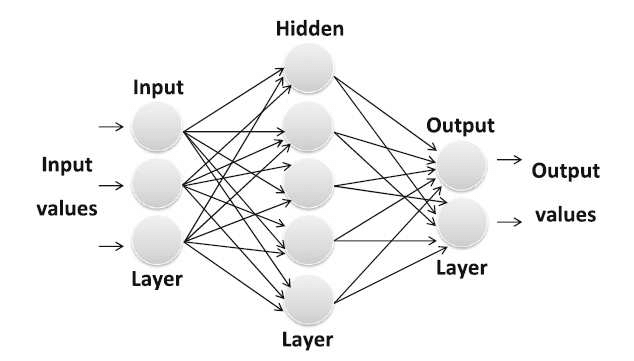
\includegraphics[scale=0.5]{Figures/MLP.png}
       \caption[MLP classifier]{MLP classifier}
       \label{fig:my_label}
   \end{figure}
   
   
\subsection{Logistic Regression}

  Logistic regression is a classification algorithm used to assign observations to a discrete set of classes. Unlike linear regression which outputs continuous number values, logistic regression transforms its output using the logistic sigmoid function to return a probability value which can then be mapped to two or more discrete classes.
  
  Logistic Regression could help use predict whether the student passed or failed. Logistic regression predictions are discrete (only specific values or categories are allowed). We can also view probability scores underlying the model’s classifications.
  
       \underline{Types of Logistic Regression}:
       \begin{enumerate}
           \item Binary: Target variable can have only 2 possible types: “0” or “1” which may represent “win” vs “loss”, “pass” vs “fail”, “dead” vs “alive”, etc.
           \item Multinomial: Target variable can have only 2 possible types: “0” or “1” which may represent “win” vs “loss”, “pass” vs “fail”, “dead” vs “alive”, etc.
           \item Ordinal: It deals with target variables with ordered categories. For example, a test score can be categorized as:“very poor”, “poor”, “good”, “very good”. Here, each category can be given a score like 0, 1, 2, 3.
       \end{enumerate}
       
\newpage
\section{Proposed CNN Model}

In machine learning, a convolutional neural network (CNN, or ConvNet) is a class of deep, feed-forward artificial neural networks that have successfully been applied to analyzing visual imagery. CNNs use a variation of multilayer perceptron designed to require minimal preprocessing. They are also known as shift invariant or space invariant artificial neural networks (SIANN), based on their shared-weights architecture and translation in variance characteristics. CNN was used to achieve some breakthrough results and win well-known contests. The application of convolutional layers consists in convolving a signal or an image with kernels to obtain feature maps. So, a unit in a feature map is connected to the previous layer through the weights of the kernels. The weights of the kernels are adapted during the training phase by back propagation, in order to enhance certain characteristics of the input. Since the kernels are shared among all units of the same feature maps, convolutional layers have fewer weights to train than dense FC layers, making CNN easier to train and less prone to overfitting. Moreover, since the same kernel is convolved over the entire image, the same feature is detected independently of the locating—translation in variance. By using kernels, information of the neighborhood is taken into account, which is a useful source of context information. Usually, a non-linear activation function is applied to the output of each neural unit.
If we stack several convolutional layers, the extracted features become more abstract with the increasing depth. The first layers enhance features such as edges, which are aggregated in the following layers as motifs, parts, or objects. The following concepts are important in the context of CNN:

\begin{enumerate}
    \item Initialization: It is important to achieve convergence. To achieve faster convergence Xavier initialization. With this, the activations and the gradients are maintained at controlled levels, otherwise, back-propagated gradients could vanish or explode.
    \item Pooling: It combines spatially nearby features in the feature maps. This combination of possibly redundant features makes the representation more compact and invariant to small image changes, such as insignificant details; it also decreases the computational load of the next stages. To join features, it is more common to use max-pooling or average-pooling.
    \item Regularization: It is used to reduce overfitting. Dropout is applied in the FC layers. In each training step, it removes nodes from the network with probability. In this way, it forces all nodes of the FC layers to learn better representations of the data, preventing nodes from co-adapting to each other. At test time, all nodes are used. Dropout can be seen as an ensemble of different networks and a form of bagging since each network is trained with a portion of the training data.
    \item Data Augmentation: It can be used to increase the size of training sets and reduce overfitting. Since the class of the patch is obtained by the central voxel, we restricted the data augmentation to rotating operations. Some authors also consider image translations, but for segmentation, this could result in attributing a wrong class to the patch. Proposed method increased our data set during training by generating new patches through the rotation of the original patch. In our proposal, we used angles a multiple of 90, although another alternative will be evaluated.
    \item Loss Function: It is the function to be minimized during training. We used the Categorical Cross-entropy
    7) Architecture: We aim at a reliable segmentation method; however, brain tumors present large variability in intra- tumoral structures, which makes the segmentation a challenging problem. To reduce such complexity, we designed a CNN and tuned the intensity normalization transformation for each tumor grade—LGG and HGG.
    Performance
    
    We used the U-Net Architecture for the above steps. The architecture is described as follows:
    
    \begin{figure}[h!]
       \centering
       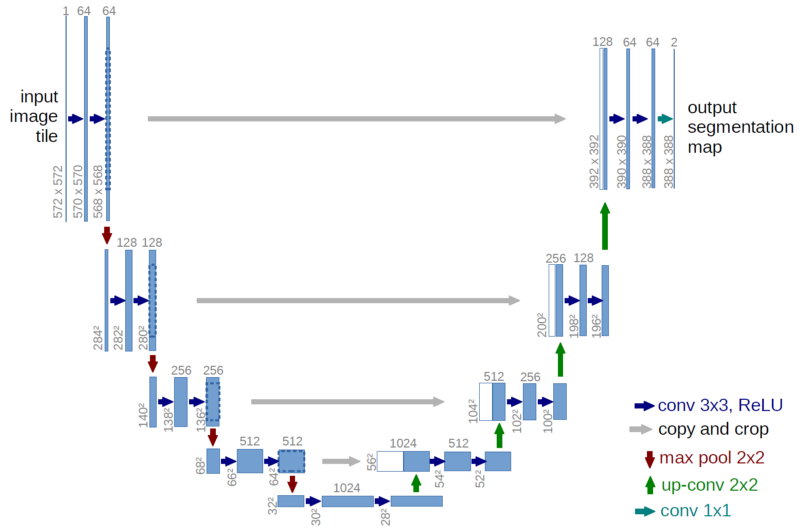
\includegraphics[scale=0.5]{Figures/unet.png}
       \caption[UNet Architecture]{UNet Architecture}
       \label{fig:UNet Architecture}
   \end{figure}
   
   The architecture looks like a ‘U’ which justifies its name. This architecture consists of three sections: The contraction, The bottleneck, and the expansion section. The contraction section is made of many contraction blocks. Each block takes an input applies two 3X3 convolution layers followed by a 2X2 max pooling. The number of kernels or feature maps after each block doubles so that architecture can learn the complex structures effectively. The bottommost layer mediates between the contraction layer and the expansion layer. It uses two 3X3 CNN layers followed by 2X2 up convolution layer.

    But the heart of this architecture lies in the expansion section. Similar to contraction layer, it also consists of several expansion blocks. Each block passes the input to two 3X3 CNN layers followed by a 2X2 upsampling layer. Also after each block number of feature maps used by convolutional layer get half to maintain symmetry. However, every time the input is also get appended by feature maps of the corresponding contraction layer. This action would ensure that the features that are learned while contracting the image will be used to reconstruct it. The number of expansion blocks is as same as the number of contraction block. After that, the resultant mapping passes through another 3X3 CNN layer with the number of feature maps equal to the number of segments desired.
    
    \subsection{Loss calculation in UNet}
    UNet uses a rather novel loss weighting scheme for each pixel such that there is a higher weight at the border of segmented objects. This loss weighting scheme helped the U-Net model segment cells in biomedical images in a discontinuous fashion such that individual cells may be easily identified within the binary segmentation map.

    First of all pixel-wise softmax applied on the resultant image which is followed by cross-entropy loss function. So we are classifying each pixel into one of the classes. The idea is that even in segmentation every pixel have to lie in some category and we just need to make sure that they do. So we just converted a segmentation problem into a multi-class classification one and it performed very well as compared to the traditional loss functions.

    \subsection{Training}
    The input images and their corresponding segmentation maps are used to train the network with the stochastic gradient descent implementation of Caffe [6]. Due to the unpadded convolutions, the output image is smaller than the input by a constant border width. To minimize the overhead and make maximum use of the GPU memory, we favor large input tiles over a large batch size and hence reduce the batch to a single image. Accordingly we use a high momentum (0.99) such that a large number of the previously seen training samples determine the update in the current optimization step.
    
    \subsection{Data Augmentation}
    Data augmentation is essential to teach the network the desired invariance and robustness properties, when only few training samples are available. In case of microscopical images we primarily need shift and rotation invariance as well as robustness to deformations and gray value variations. Especially random elas- tic deformations of the training samples seem to be the key concept to train a segmentation network with very few annotated images. We generate smooth deformations using random displacement vectors on a coarse 3 by 3 grid. The displacements are sampled from a Gaussian distribution with 10 pixels standard deviation. Per-pixel displacements are then computed using bicubic interpola- tion. Drop-out layers at the end of the contracting path perform further implicit data augmentation.

    
\end{enumerate}



      
 